\documentclass[a4paper]{article}
\usepackage{fullpage}
\usepackage{enumerate}
\usepackage[T1,T2A]{fontenc}
\usepackage[utf8]{inputenc}
\usepackage[bulgarian]{babel}
\usepackage{soul}
\usepackage{graphicx}
\usepackage{usecases}

\begin{document}

\title{Информационна система на агенция за недвижими имоти\\Доклад за индивидуална работа по проекта}
\author{Александър Велин 71512 \\\emph{(екип $\pi \approx 3.1$)}}

\maketitle

\clearpage

%\tableofcontents

%\clearpage

\section*{Интервюта}

Участвах и в двете проведени две интервюта с Борислав Арнаудов (собственик на стартираща агенция за недвижими имоти) за изясняване изискванията към системата:
\begin{itemize}
\item на 2016-03-18 от 16:00 до 17:30 в зала 01 на ФМИ
\item на 2016-04-01 от 09:00 до 10:30 в офиса на САП България
\end{itemize}

\section*{Contextual Design модел}

От идентифицираните на базата на събраната информация роли, разработих модел на дейностите на Одитор.

\begin{figure}[h]
\centering
\label{auditor}
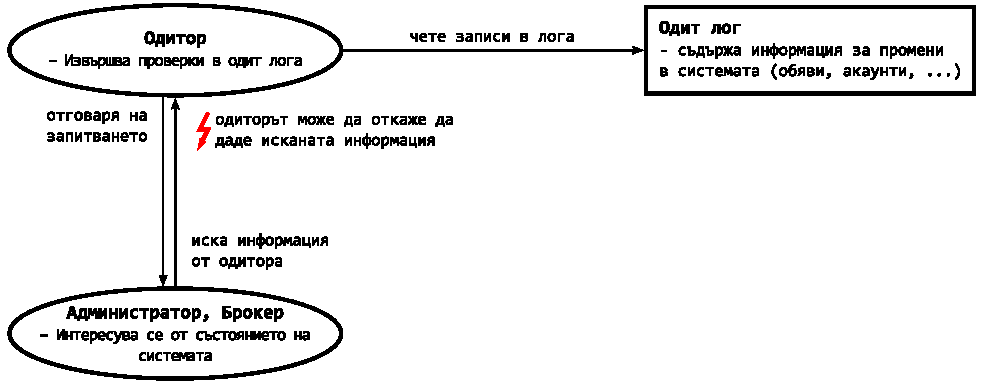
\includegraphics[scale=0.85]{flow-auditor-small}
\caption{Flow модел за Одитор}
\end{figure}

%\emph{Моделът е показан на Фигура 1.} 

В системата съсществува вграден акаунт за одитор, който има права само да чете одит лога. При нужда от информация за настъпила промяна в системата (за даден акаунт, обява и т.н.), брокерите, администраторът, собственикът на фирмата могат да поискат от одитора информация защо е настъпила промяната. 
	
\emph{Заб. Одиторът може да откаже достъп до поисканата информация. Правилата за допуск са извън обхвата на системата.}

\clearpage
\section*{Use case модел}

На базата на идентифицираните потребителски случаи, участвах в разработката на Модела на потребителските случаи:

        \begin{figure}[h]
        \centering
        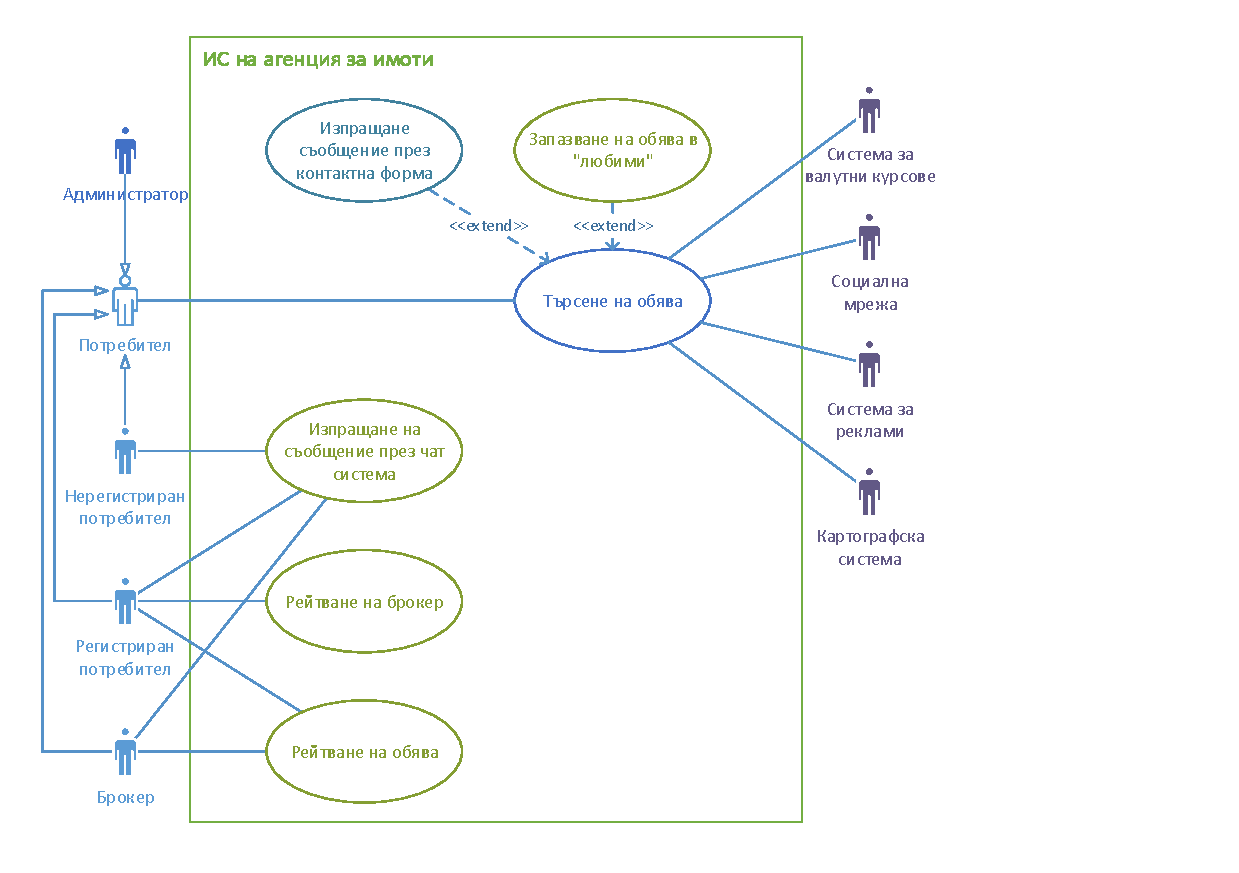
\includegraphics[scale=1]{uc2a}
        \caption{Модел на потребителските случаи, свързани с основните функционалности на системата (от гледна точка на потребителите)}
        \end{figure}

\clearpage

        \begin{figure}[h]
        \centering
        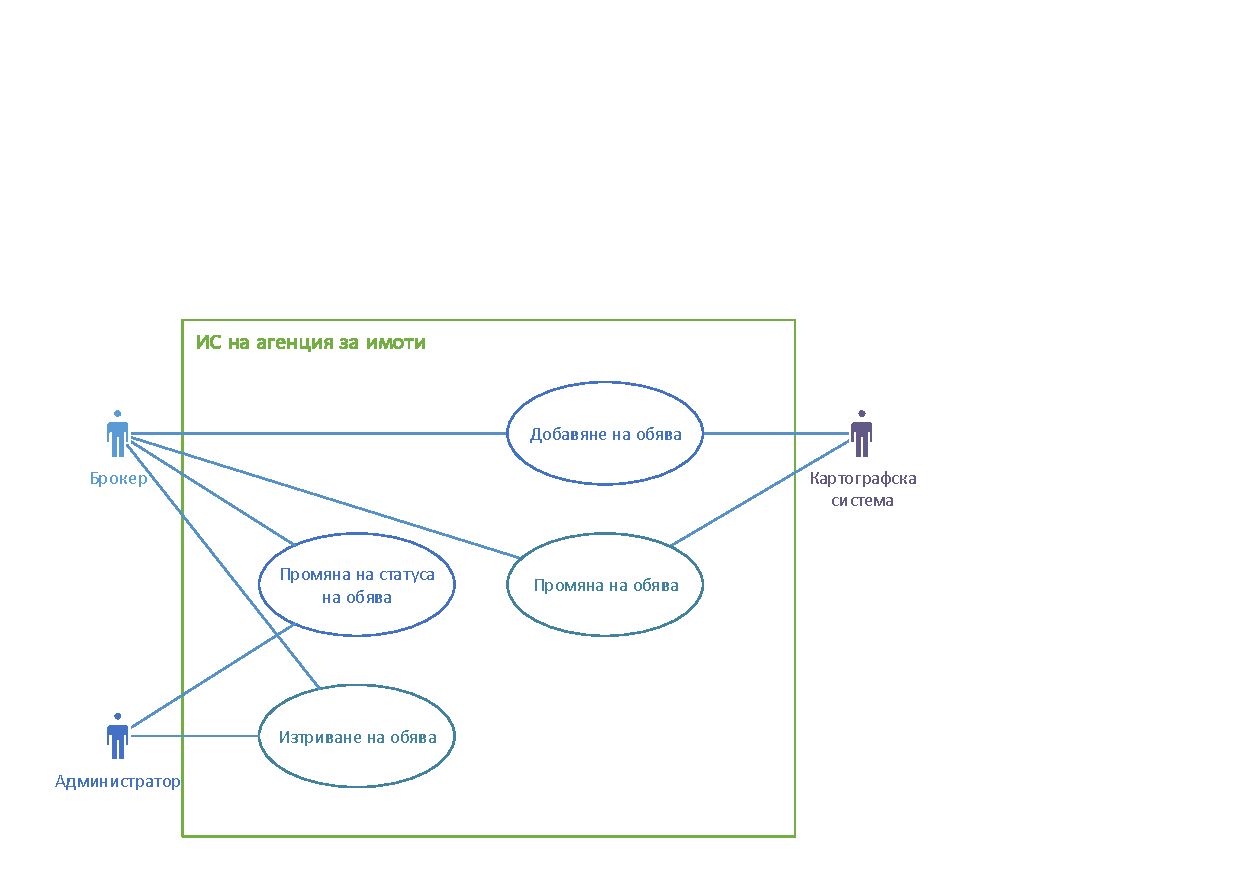
\includegraphics[scale=1]{uc2b}
        \caption{Модел на потребителските случаи, свързани с обяви за имоти (от гледна точка на брокерите)}
        \end{figure}

\clearpage

        \begin{figure}[h]
        \centering
        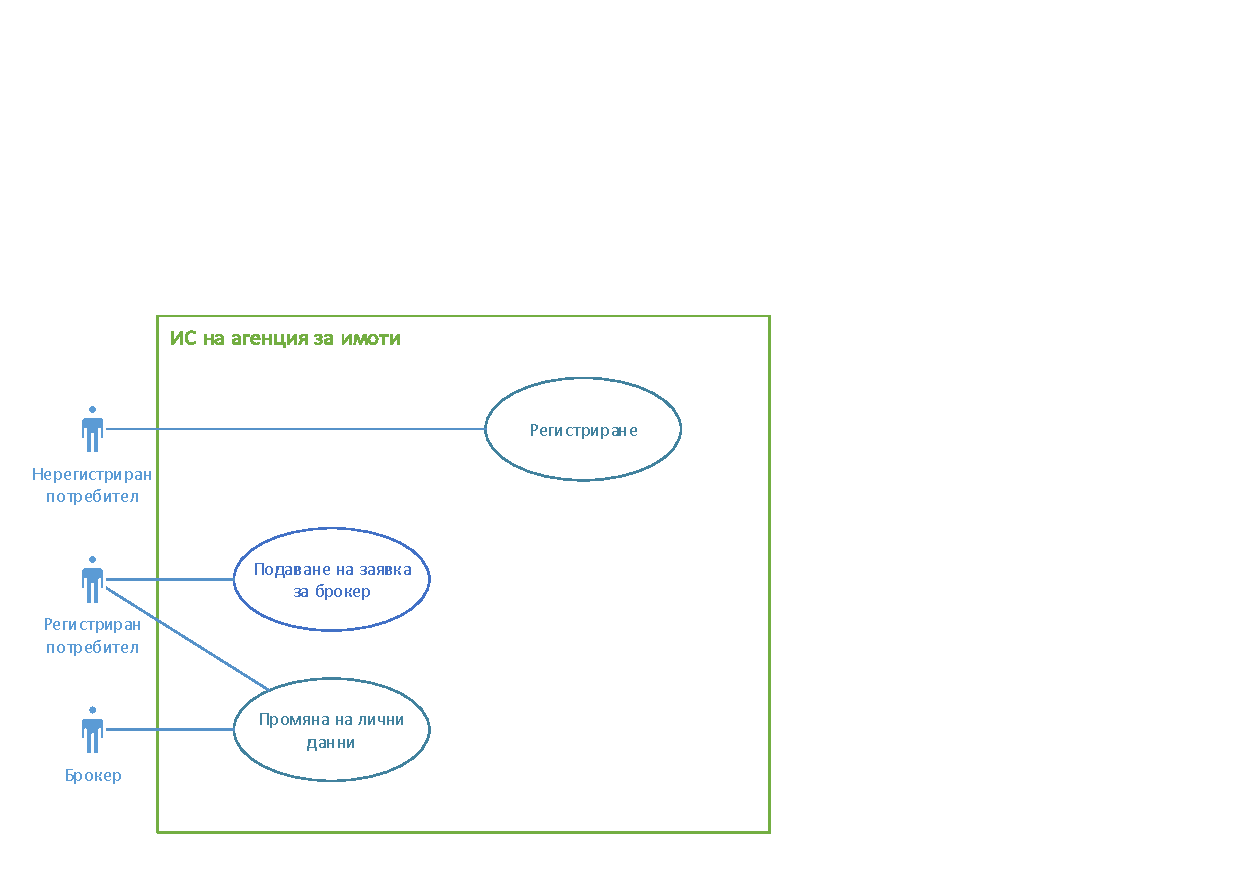
\includegraphics[scale=1]{uc2c}
        \caption{Модел на потребителските случаи, свързани с акаунти на потребители}
        \end{figure}

\clearpage

        \begin{figure}[h]
        \centering
        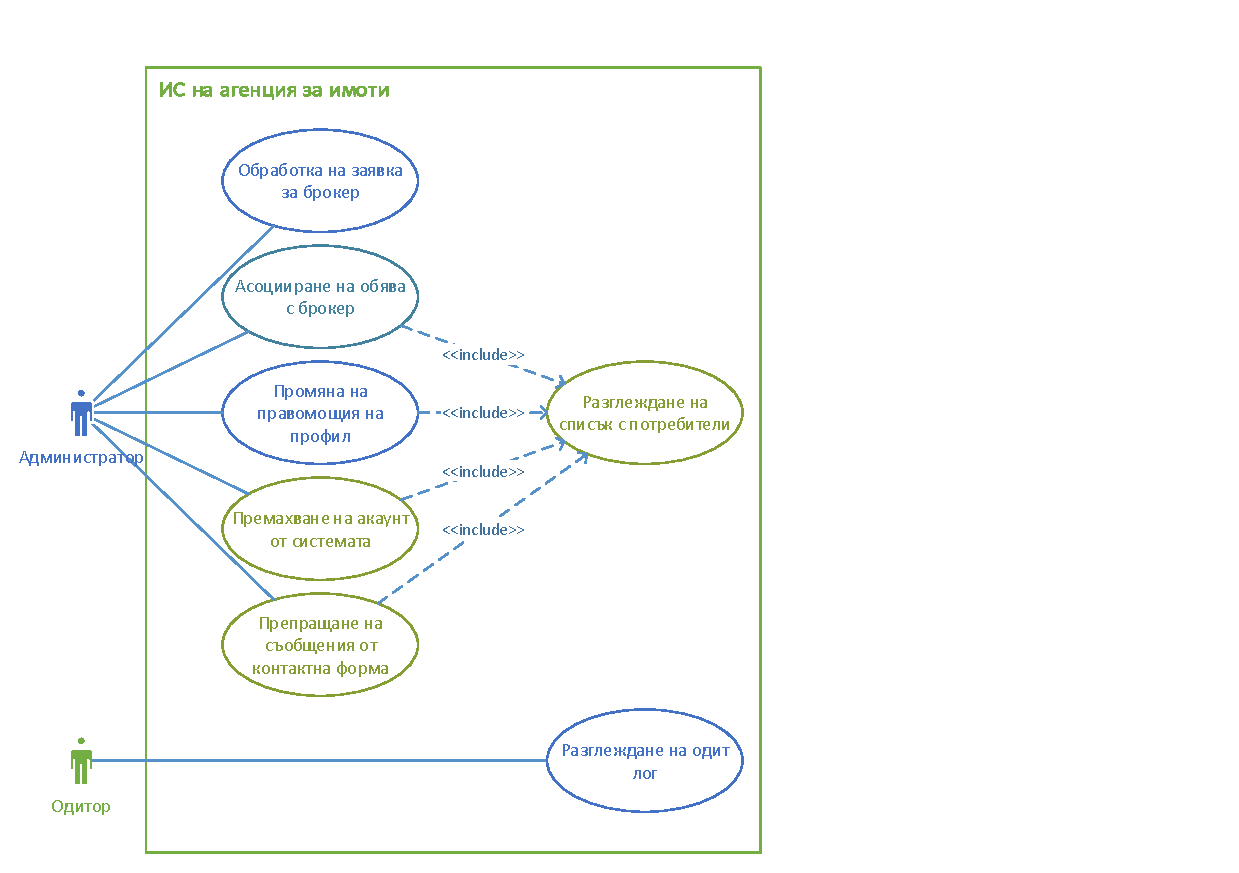
\includegraphics[scale=1]{uc2d}
        \caption{Модел на потребителските случаи, свързани с административни дейности}
        \end{figure}

\clearpage
\section*{Шаблон за пълно описание на потребителските случаи}

Съгласно изискванията за част II на проекта, разработих шаблон за пълно описание на потребителските случаи.

\begin{usecase}
\addtitle{Потребителски случай \emph{<номер>}}{\emph{<име на потребителският случай>}} 
\addfield{Ниво:}{\emph{<user-goal или subfunction>}}
\addfield{Основен актьор:}{\emph{<основен актьор>}}
\additemizedfield{Заинтересовани лица и техните интереси:}{
	\item \emph{<заинтересовано лице и интереси>}
}
\additemizedfield{Предусловия:}{
	\item \emph{<предусловие>}
}
\additemizedfield{Следусловия:}{
	\item \emph{<следусловие>}
}
\addfield{Тригер:}{\emph{<стартиране>}}
\addscenario{Основен успешен сценарий:}{
	\item \emph{<стъпка>}
	\item \emph{<стъпка>}
}
\addscenario{Алтернативни сценарии:}{
        \item[2.a] \emph{<Алтернативна стъпка на такава от основния сценарий>}:
                \begin{enumerate}
                \item[1.] \emph{<стъпка от алтернативния сценарий>}
                \item[2.] \emph{<стъпка от алтернативния сценарий>}                
                \end{enumerate}
        \item[5.a] \emph{<Алтернативна стъпка на такава от основния сценарий>}:
                \begin{enumerate}
                \item[1.] \emph{<стъпка от алтернативния сценарий>}
                \item[2.] \emph{<стъпка от алтернативния сценарий>}                
                \end{enumerate}
}                
\additemizedfield{Специални изисквания:}{
		\item \emph{<Незадължително поле за специални изисквания>}
}
\addfield{Честота на настъпване:}{\emph{<колко често се случва потребителският случай>}}
\addfield{Коментари:}{\emph{<Незадължително поле за коментари и въпроси>}}
\end{usecase}

\clearpage
\section*{Пълно описание на потребителските случаи}

От идентифицираните потребителски случаи, описах следните два в пълен (fully dressed) формат:

\subsection*{Разглеждане на одит лог} % А5

\begin{usecase}
\addtitle{Потребителски случай A-5}{Разглеждане на одит лог} 
\addfield{Ниво:}{user-goal}
\addfield{Основен актьор:}{Одитор}
\additemizedfield{Заинтересовани лица и техните интереси:}{
	\item Администратор, Брокери, Бизнес: Интересуват се защо данните в системата са в определено състояние
	\item Одитор: иска да види какви събития са отразените в одит лога събития, настъпили в системата, които биха могли да обяснят текущото ѝ състояние
}
\additemizedfield{Предусловия:}{
	\item Само брокерите, администраторът и собственикът на фирмата могат да поискат справка от одитора
	\item Искането към одитора трябва да отговаря на установените правила за допуск до информация. (Извън обхвата на системата.)
	\item Одиторът е логнат в системата
}
\addfield{Следусловия:}{Ако информация, отговаряща на критериите за търсене, дефинирани от одитора съществува, то системата трябва да я предостави на одитора.}
\addfield{Тригер:}{Одиторът избира достъп до функционалност ``Разглеждане на одит лог''}
\addscenario{Основен успешен сценарий:}{
	\item Системата предоставя възможност за дефиниране на ограничения по времеви интервал, username, IP адрес, тип на действието, субект на действието
	\item Одиторът променя критериите за търсене в одит лога
	\item Системата предоставя всички записи, отговарящи на текущите критерии за търсене в одит лога, чрез подмножества (страници)
	\item Одиторът разглежда предоставената информация
}
\addscenario{Алтернативни сценарии:}{
        \item[4.a] Одиторът променя критериите за търсене в одит лога
                \begin{enumerate}[1.]
                \item Системата препраща потребителя към стъпка 3 от основния сценарий
                \end{enumerate}
}                
\additemizedfield{Специални изисквания:}{
        \item Информацията в одит лога не може да се променя от никого
        \item Системата премахва от одит лога информация, по-стара от 6 месеца.
}
\addfield{Честота на настъпване:}{Рядко, не се очаква по-често от 10-тина пъти седмично.}
\end{usecase}

\subsection*{Разглеждане на списък с потребители} % C7

\begin{usecase}
\addtitle{Потребителски случай C-7}{Разглеждане на списък с потребители} 
\addfield{Ниво:}{subfunction}
\addfield{Основен актьор:}{Администратор}
\additemizedfield{Заинтересовани лица и техните интереси:}{
	\item Администратор: Иска да избере конкретен потребител на системата
}
\additemizedfield{Предусловия:}{
	\item Администраторът да е логнат в системата
	\item Да съществуват други акаунти в системата освен вградените Администратор и Одитор
}
\addfield{Следусловия:}{Системата ``знае'' дали и кой потребител е избрал Администраторa}
\addfield{Тригер:}{Администраторът избира достъп до функционалност за разглеждане на списък с потребители}
\addscenario{Основен успешен сценарий:}{
	\item Системата предоставя списък с всички регистрирани потребители, отговарящи на текущите критерии за търсене на потребители (при нужда - разделени на страници)
	\item Администраторът избира потребител
}
\addscenario{Алтернативни сценарии:}{
        \item[2.a] Администраторът променя критериите за търсене на потребители
                \begin{enumerate}[1.]
                \item Системата препраща Администратора към стъпка 1 от оригиналния сценарий
                \end{enumerate}
        \item[2.b] Администраторът не избира потребител
}                
\addfield{Специални изисквания:}{Системата позволява избиране само на акаунти тип Регистриран потребител и Брокер, без сервизните Администратор и Одитор}
\addfield{Честота на настъпване:}{Очаквано -- няколко пъти седмично.}
%\addfield{Коментари:}{\emph{<Незадължително поле за коментари и въпроси>}}
\end{usecase}



\clearpage
\section*{Домейн модел}

На базата на участието ми в определянето на домейн модела, създадох следната диаграма:

\begin{center}
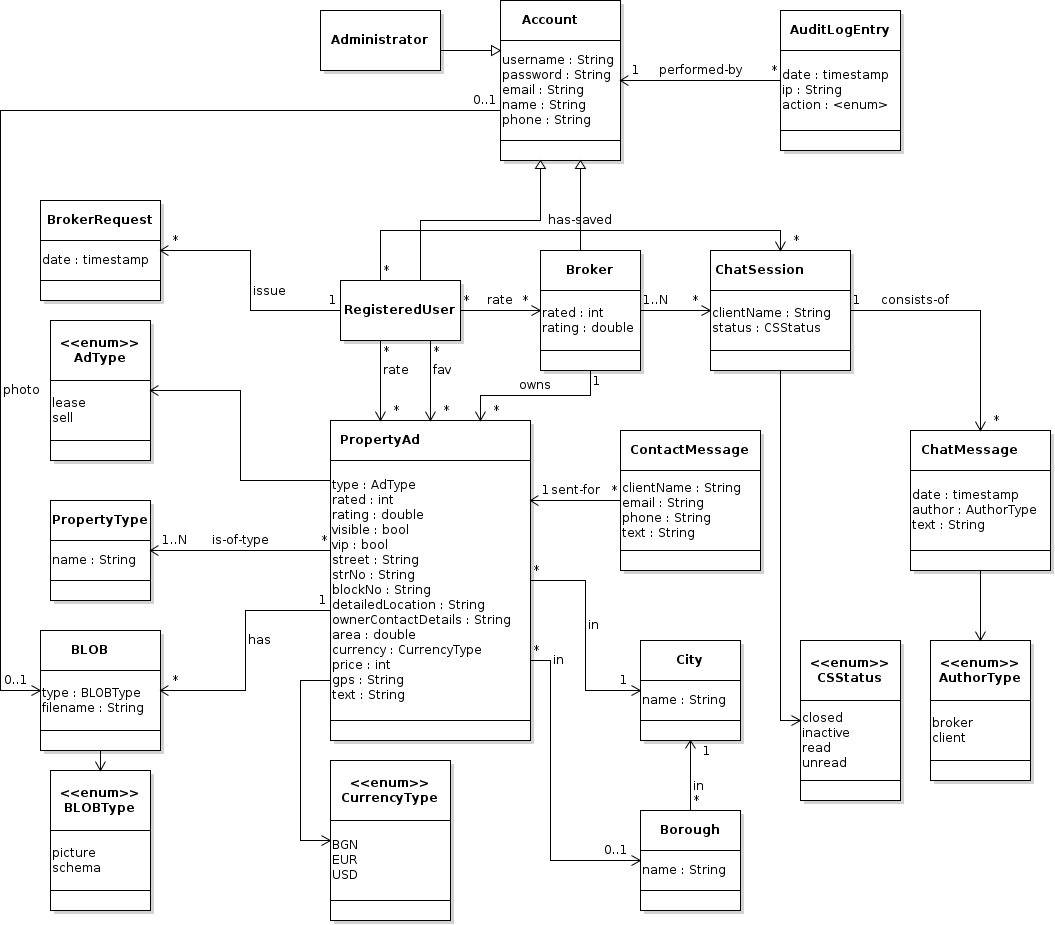
\includegraphics[scale=0.48,keepaspectratio=true]{domain-model}
\end{center}

Класът Account съдържа атрибути за потребителско име, парола, email адрес, име и телефонен номер. Той се наследява от класовете Administrator, RegisteredUser и Broker. Всеки акаунт би могъл да е асоцииран с не повече от един обект от клас BLOB, като асоциацията представлява снимка на съответният потребител.

Класът BLOB представя съществуващи двоични файлове в системата. Той има атрибути за тип на файла (type - изброен тип, picture или schema) и име на файла (filename).


Когато регистриран потребител подаде заявка, че иска да стане брокер, се създава обект от клас BrokerRequest (асоцииран с RegisteredUser-a), който обект съществува до момента на одобряване или отхвърляне на заявката.

Класът Broker съдържа допълнителни атрибути:
\begin{itemize}
\item rating -- натрупан до момента рейтинг на брокера
\item rated -- брой на гласовете за рейтинг
\end{itemize}

При започване на чат сесия, в системата се създава обект от клас ChatSession (асоцииран с участващите в сесията Broker-и), който има атрибути:
\begin{itemize}
\item clientName -- име, с което потребителят участва в чат сесията
\item status -- изброен тип с възможните състояния на сесията (closed, inactive, read, unread)
\end{itemize}
Сесията е асоциирана с обекти ChatMessage, които имат атрибути date, author (изброен тип -- broker или client), и text на самото съобщение.

Обектите от клас City (с атрибут name) дефинират на населените места, които подържа системата. Подобен е и класът Borough (с атрибут name), който дефинира квартали. Всеки обект от клас Borough е асоцииран с град, в който се намира.

Класът ContactMessage описва дадено съобщение, изпратено през формата за контакт. Съдържа атрибути за име клиента (clientName), email адрес на клиента (email), телефон за обратна връзка (phone) и самото текстово съобщение (text).

Основен е класът PropertyAd, който съдържа информация за обява в системата. Основни негови атрибути са:
\begin{itemize}
\item type -- тип на обявата, изброен тип (lease/sell)
\item area -- застроена площ на имота
\item price -- цена на имота
\item currency -- валута на цената, изброен тип (BGN/EUR/USD)
\item rating -- натрупан до момента рейтинг на обявата
\item rated -- брой на гласовете за рейтинг
\item visible -- bool, който дефинира дали обявата е публично видима
\item vip -- bool, който дефинира дали обявата е нормална или vip
\end{itemize}
Класът участва в следните асоциации:
\begin{itemize}
\item с BLOB -- дефинира снимки и скици на имота
\item с City -- дефинира в кой населен пункт се намира имота
\item с Borough -- дефинира в кой квартал се намира имота
\item с ContactMessage -- всяко изпратено през контакт формата съобщение се отнася за конкретна обява в системата
\end{itemize}

Действията, променящи системата създават обекти от клас AuditLogEntry, които са асоциирани с акаунта, извършил действието и съдържат атрибути за дата (date), IP адрес (ip) и извършено действие (action).

\clearpage
\section*{Разпределение на времето}

В таблицата е описано времето (в минути) за работата по различните части и задачи на проекта.

\begin{table}[h]
\centering
\begin{tabular}{|l|l|l|l|l|l|l|l|l|l|l|}
\hline
                        	& 71512 \\ \hline
Интервю 1               	& 90    \\ \hline
Интервю 2               	& 90    \\ \hline
Транскрибиране 1        	& 90    \\ \hline
Транскрибиране 2        	& 120   \\ \hline
Записки 1               	& 0     \\ \hline
Записки 2               	& 0     \\ \hline
Резюме 1                	& 360   \\ \hline
Резюме 2                	& 120   \\ \hline
Уточняване на модели    	& 60    \\ \hline
Работа по CD модели     	& 120   \\ \hline
Подготовка на Доклад I  	& 540   \\ \hline
\hline
Коригиране на I-ва част		& 0   	\\ \hline
Визия						& 15   	\\ \hline
Use Case модел				& 90   	\\ \hline
Списък Актьори				& 15   	\\ \hline
Списък UC (brief)			& 30   	\\ \hline
Шаблон за UC				& 30   	\\ \hline
Fully dressed UC			& 30   	\\ \hline
Нефункционални изисквания	& 10   	\\ \hline
Речник						& 20   	\\ \hline
Review						& 180  	\\ \hline
Подготовка на Доклад II		& 450  	\\ \hline
\hline
Коригиране на II-ра част	& 90   	\\ \hline
Use Case модел				& 180  	\\ \hline
Пълен списък UC				& 0   	\\ \hline
Fully dressed UC			& 120  	\\ \hline
Домейн модел				& 450  	\\ \hline
UML диаграми				& 0   	\\ \hline
Примерен план на проекта	& 60   	\\ \hline
Подготовка на Доклад III	& 390  	\\ \hline
\textbf{Общо}				& 3750 	\\ \hline
\end{tabular}
\end{table}

\end{document}
